\chapter{The lock-in amplifier}\label{lokkin}
	\section{Basic theory}
A lock-in amplifer is a device which is useful for measuring the amplitude and phase of a signal. The output will typically be a DC voltage which is proportional to the input amplitude. The device has two inputs as shown in \cref{lockin1}. One is the input signal that is to be measured, and the other is a reference. The reference should have the exact same frequency as the input. This signal is usually a sync-signal originating from the same source as the input signal. The input signal is first passed through an amplifier of gain $g$, which is adjustable and is used to control the sensitivity of the lock-in. The reference signal instead is led through a sine-former, i.e.  a block consisting of many components which transform the signal to ensure it has sinusoidal form and a specific predetermined amplitude.

\begin{figure}[!hbt]\centering
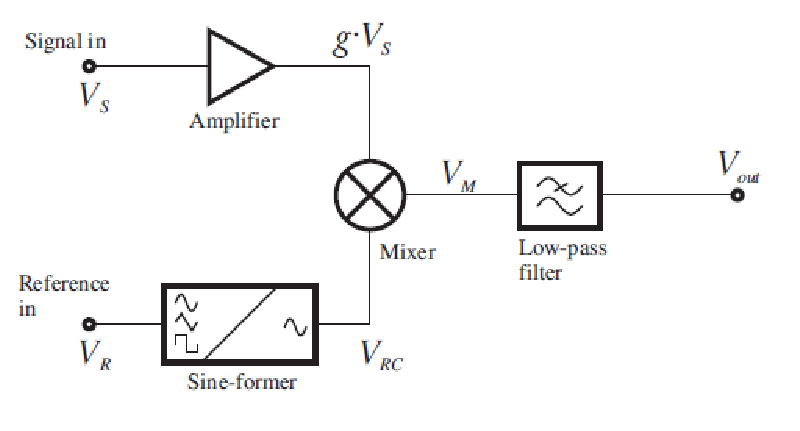
\includegraphics[width=\linewidth, draft=\foto]{eps/lockin1.eps}
\caption{Block scheme of a lock-in amplifier.}
\label{lockin1}
\end{figure}

The following \cref{sinusoidal} states the input signal if we assume it is sinusoidal\footnote{Of course this is never the case, but thanks to Fourier decomposition we can think of the generic signal as a sum of sinusoidal components.}, with amplitude $K$ and frequency $f$, while \cref{reference} states the reference signal after it has passed through the sine-former, and assuming it has the exact same frequency $f$ as the input signal
\begin{align}
V_{\mai{s}}=K\cos[2\pi ft+\phi_{\mai{s}}]
\label{sinusoidal}\\
V_{\mai{rc}}=\cos[2\pi ft+\phi_{\mai{r}}]
\label{reference}
\end{align}
The mixer then combines these two signals by multiplying them, giving
\begin{align}
V_{\mai{m}}&=Kg\cos[2\pi ft+\phi_{\mai{s}}]\cos[2\pi ft+\phi_{\mai{r}}]\nonumber\\
&=\frac{1}{2}Kg\left(\cos[\phi_{\mai{s}}-\phi_{\mai{r}}]+\cos[2\pi\cdot2ft+\phi_{\mai{s}}+\phi_{\mai{r}}]\right)\label{mixer}
\end{align}

As can be seen in \cref{mixer}, the result consists of two frequency components. One at zero (DC), and one at the double frequency. If the low pass filter is set correctly the double frequency component will be completely removed, and the output is therefore as stated by
\mate
V_{\mai{out}}=\frac{1}{2}Kg\cos\left[\phi_{\mai{s}}-\phi_{\mai{r}}\right]
\atem

We can see that the output is a DC voltage which is proportional to the signal amplitude $K$. The amplifier gain $g$ is such that, when assuming  $\phi_{\mai{s}}=\phi_{\mai{r}}$, the output is 10V if the RMS-value of the input signal is the same as the sensitivity-setting. For lower input signals, the output is proportionally lower, and a higher input will overload the lock-in. The sensitivity is a quantity which can be controlled from the front panel.

\mate
g=\frac{10V\cdot\sqrt{2}}{\mbox{sensitivity}}
\atem

	\section{Dual lock-in amplifier}
The lock-in amplifier has instead two mixers with dedicated low pass filters. One of these mixers multiplies the reference and the input signal like before, and the other one multiplies the input signal with the reference phase shifted by 90\textdegree. \cref{lockin2} illustrates this principle.

\begin{figure}[!hbt]\centering
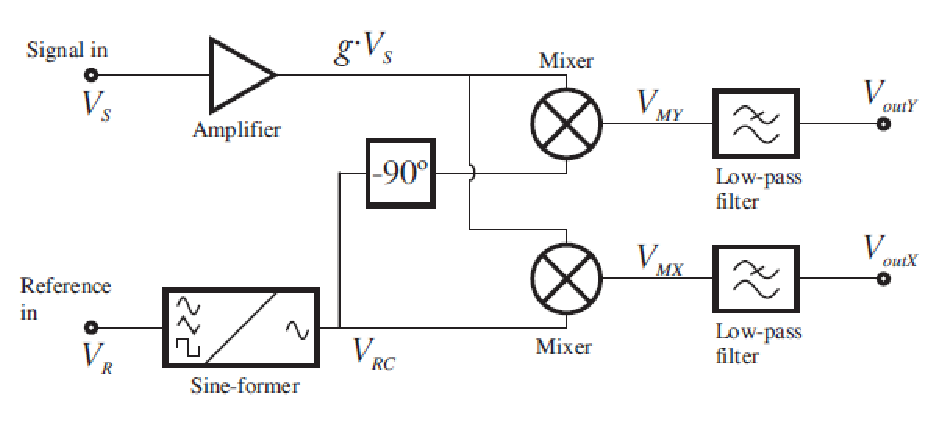
\includegraphics[width=\linewidth, draft=\foto]{eps/lockin2.eps}
\caption{A dual lock-in amplifier}
\label{lockin2}
\end{figure}

The two outputs then become

\begin{align}
V_{\mai{out}}^{\mai{x}}&=\frac{1}{2}Kg\cos\left[\phi_{\mai{s}}-\phi_{\mai{r}}\right]
\\
V_{\mai{out}}^{\mai{y}}&=\frac{1}{2}Kg\sin\left[\phi_{\mai{s}}-\phi_{\mai{r}}\right].
\end{align}

$V_{\mai{out}}^{\mai{x}}$ is called the in phase component of the output, while $V_{\mai{out}}^{\mai{y}}$ is called the out of phase component. For convenience it could be useful to define a new complex quantity $V_{\mai{out}}^{\mai{cp}}$ like

\mate
V_{\mai{out}}^{\mai{cp}}=V_{\mai{out}}^{\mai{x}}+iV_{\mai{out}}^{\mai{y}}
\atem

No matter what the phase difference between the input and the reference is, the magnitude of $V_{\mai{out}}^{\mai{cp}}$ can now be used to find the amplitude of the input signal at frequency $f$ .

	\section{Low-pass filter}

The low pass filters in \cref{lockin1,lockin2} are supposed to remove the double frequency component in \cref{mixer}. In addition these filters may remove a lot of noise. \cref{lockin3} shows such an example. Here the mixing process causes a shift in the spectrum such that the desired signal is shifted to $f=0$ (DC). The dotted line represents the frequency response of the filter, and should be multiplied with the input signal to give the output. All the noise which is not within the bandwidth of the filter is removed.

The filter is adjustable from the front panel through two parameters. One of them is the time constant $\tau$. If the input were to suddenly change, this is the time it would take before the output is adjusted to 63\% of this change. The second parameter is the number of such filters. Between one and four filters with the same time constant $\tau$ can be cascaded to form a sharper filter.

\begin{figure}[!hbt]\centering
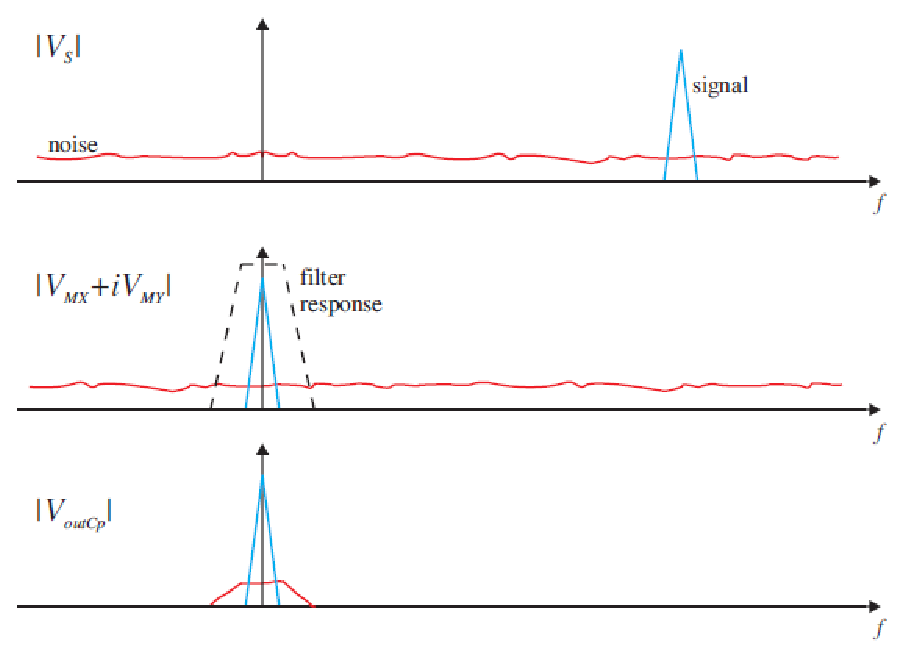
\includegraphics[width=\linewidth, draft=\foto]{eps/lockin3.eps}
\caption{The low pass filter removes all the noise which is not within the bandwidth of the filter.}
\label{lockin3}
\end{figure}
